\documentclass[12pt,a4paper]{report}

\usepackage[margin=1in]{geometry}
\usepackage[T1]{fontenc}
\usepackage[utf8]{inputenc}
\usepackage{lmodern}
\usepackage{setspace}
\usepackage{hyperref}
\usepackage{graphicx}
\usepackage{booktabs}
\usepackage{longtable}
\usepackage{tabularx}
\usepackage{array}
\usepackage{enumitem}
\usepackage{xcolor}
\usepackage{listings}
\usepackage{float}

\hypersetup{
    colorlinks=true,
    linkcolor=blue!60!black,
    urlcolor=blue!60!black,
    pdftitle={AutoTrade Project Report},
    pdfauthor={Rahul Motors},
    pdfsubject={Database Management Systems Project Report}
}

\setstretch{1.2}
\setlength{\parskip}{0.4em}
\setlength{\parindent}{0pt}

\definecolor{codebg}{RGB}{248,248,248}
\definecolor{codecomment}{RGB}{0,128,0}
\definecolor{codekeyword}{RGB}{0,0,180}
\definecolor{codestring}{RGB}{163,21,21}

\lstdefinestyle{projectcode}{
    backgroundcolor=\color{codebg},
    basicstyle=\ttfamily\small,
    breaklines=true,
    columns=fullflexible,
    commentstyle=\color{codecomment},
    frame=single,
    keywordstyle=\color{codekeyword}\bfseries,
    numbers=left,
    numbersep=8pt,
    numberstyle=\tiny\color{gray},
    showstringspaces=false,
    stringstyle=\color{codestring},
    tabsize=2
}

\lstset{style=projectcode}

% Custom Command for Times New Roman-like look for title if needed
\newcommand{\tnr}{\fontfamily{ptm}\selectfont}

\begin{document}

\begin{titlepage}
  \centering
  \vspace*{1cm}
  {\tnr\fontsize{24}{28}\selectfont \textbf{AUTOTRADE: VEHICLE BUYING AND SELLING PLATFORM}} \\[1.5cm]
  
  {\tnr\fontsize{18}{22}\selectfont Project Report} \\[0.5cm]
  {\tnr\fontsize{16}{20}\selectfont submitted in partial fulfilment for the degree of} \\[0.3cm]
  {\tnr\fontsize{16}{20}\selectfont Masters of Technology} \\[0.3cm]
  {\tnr\fontsize{16}{20}\selectfont Under the Faculty of Engineering} \\[1.5cm]

  {\tnr\fontsize{14}{17}\selectfont\itshape Submitted by\par}
  \vspace{0.5cm}
  {\fontsize{14}{16}\selectfont \textbf{RAHUL MOTORS} \par}
  {\fontsize{14}{16}\selectfont \textbf{ID: rahul\_motors} \par}

  \vspace{1.5cm}
  
\includegraphics[width=15.67cm,height=4.0cm]{screenshots/Picture1.jpg}

  \vspace{1.5cm}
  {\tnr\fontsize{15}{18}\selectfont
  DEPARTMENT OF COMPUTER SCIENCE AND ENGINEERING\par
  AMRITA SCHOOL OF COMPUTING,\par
  AMRITA VISHWA VIDYAPEETHAM,\par
  }

  \vfill
  {\tnr\fontsize{15}{18}\selectfont APRIL, 2026\par}
  {\tnr\fontsize{15}{18}\selectfont COIMBATORE CAMPUS\par}
\end{titlepage}

\pagenumbering{roman}
\tableofcontents
\listoftables
\listoffigures

\newpage
\pagenumbering{arabic}

\chapter{Introduction}
\section{Background}
The automotive industry is currently navigating a digital transformation where the "Vehicle Lifecycle" is no longer just a physical concern but a data-intensive journey. Traditional automotive marketplaces operate in silos: one site for buying cars, another for finding parts, and yet another for booking services. This fragmented approach leads to information gaps, especially concerning vehicle provenance (history) and service verification.

AutoTrade addresses these gaps by creating a unified ecosystem. It manages multiple categories of information: vehicle specifications, real-time inventory, user purchase history, service center interactions, spare parts logistics, and intelligent recommendations. To handle this diversity, the system moves away from single-database architecture towards a specialized Polyglot Persistence model.

\section{Problem Statement}

\paragraph{The Challenge of Verified Provenance and Fraud Prevention} 
In the traditional automotive marketplace, maintaining a transparent and immutable history of a vehicle—often referred to as provenance—is a significant hurdle. Standard relational databases struggle to trace a vehicle's multi-faceted history across disparate tables (sales, accidents, service records) without incurring heavy performance costs due to complex joins. This structural limitation makes it difficult to efficiently detect odometer fraud or verify a chain of ownership in real-time. When these records are disconnected, information gaps occur, undermining buyer trust and making it nearly impossible to verify the true "digital health" of a vehicle before a transaction.

\vspace{1em} 

\paragraph{Performance Bottlenecks in Real-Time Discovery} 
High-volume vehicle marketplaces require instantaneous filtering and search capabilities to maintain user engagement. However, traditional architectures often face significant bottlenecks when high-volume search queries for specific makes, models, and price ranges are executed against the same relational database handling active transactional orders. This "relational overhead" creates a conflict between data integrity and search speed. As the inventory scales, the time it takes to refresh a search result increases, leading to a degraded user experience where the platform becomes unresponsive during peak traffic periods.

\vspace{1em}

\paragraph{Computational Complexity of Intelligent Cross-selling} 
One of the primary limitations of a purely relational approach is the difficulty in performing the multi-hop traversals required for intelligent cross-selling and "Frequently Bought Together" logic. In a SQL environment, calculating personalized recommendations in real-time involves recursive queries and nested joins that are computationally expensive and scale poorly. This prevents marketplaces from offering the level of sophistication found in modern e-commerce, as the database cannot efficiently uncover the hidden patterns of user behavior and vehicle relationships that drive auxiliary sales of parts and services.

\vspace{1em}

\paragraph{Enforcement of Operational Integrity and Data Governance} 
Ensuring the quality and legality of marketplace listings is a continuous challenge that often fails when handled solely at the application level. Without strict enforcement at the data layer, "zombie" listings—such as vehicles that exceed a 15-year age limit or entries with invalid pricing—can bypass frontend validations and clutter the platform. This lack of automated governance leads to a "polluted" inventory that frustrates users and complicates administrative oversight. Relying on manual intervention is inefficient; instead, business rules must be embedded directly into the database architecture to ensure every listing adheres to platform standards by default.

\section{Objectives}
\begin{description}[leftmargin=0em, itemsep=1.5em]
    \item[Technical Innovation through Polyglot Architecture:] The primary objective of this project is to implement a robust polyglot persistence architecture that leverages the specialized strengths of MySQL, MongoDB, and Neo4j. By moving away from a traditional monolithic database, the system ensures high operational reliability through MySQL’s ACID-compliant transactional engine, while achieving high-speed metadata retrieval and schema flexibility via MongoDB’s document-oriented storage. Furthermore, the integration of Neo4j provides the platform with native intelligence, allowing for real-time recommendation engines and relationship mapping that would be computationally prohibitive in a standard relational environment.

    \item[Fraud Prevention and Graph-Based Provenance:] To address the pervasive issue of information asymmetry in the second-hand vehicle market, the project focuses on building a dedicated graph-based provenance engine. By utilizing Neo4j, the system maps the entire lifecycle of a vehicle—including ownership transfers, service logs, and registration updates—as a series of connected nodes and relationships. This structural transparency allows the platform to perform deep-path traversals to trace vehicle history and automatically flag mileage anomalies or suspicious patterns that suggest odometer tampering, providing a "Digital Passport" for each vehicle that significantly enhances buyer trust.

    \item[Marketplace Automation and Operational Integrity:] The third core objective is to maximize marketplace automation by embedding critical business logic directly into the data layer using MySQL Stored Procedures and Triggers. By automating inventory management, the system ensures that vehicle status updates occur instantaneously and atomically, without relying on external application-level code. Triggers are strategically implemented to enforce operational integrity, such as validating that no vehicle exceeding the 15-year age limit is listed, thereby reducing the risk of human error and ensuring the database remains a self-regulating, high-quality repository of transactional data.
\end{description}

\section{System Roles and Functionality}

\begin{description}[leftmargin=0em, itemsep=1.5em]

    \item[Admin Panel:] This administrative module provides comprehensive oversight of the entire marketplace, facilitating user moderation and high-level platform management. It utilizes integrated dashboard analytics, powered by MongoDB aggregation pipelines, to provide real-time insights into market trends, transaction volumes, and system performance metrics.

    \item[Seller Dashboard:] The seller interface is designed for streamlined inventory management, featuring an advanced vehicle listing system. It incorporates Cloudinary image integration for high-fidelity media hosting and provides real-time status tracking, ensuring sellers can monitor the lifecycle of their listings from initial post to final sale.

    \item[Buyer Experience:] The buyer-centric frontend is optimized for a seamless consumer journey, offering high-speed browsing and filtering capabilities. It prioritizes transparency through detailed fraud reports generated by the Neo4j provenance engine, while integrating comprehensive modules for spare part purchasing and service center booking.

\end{description}

\chapter{Requirements Analysis}
\section{Functional Requirements}
\begin{longtable}{p{0.25\textwidth} p{0.68\textwidth}}
\toprule
\textbf{Module} & \textbf{Functional Requirements} \\
\midrule
\endhead
Authentication & Role-based login (User, Service Center, Admin) with secure session management. \\
Vehicle Inventory & CRUD operations for car listings, including automated age validation and price-range checks. \\
Discovery Engine & Multi-parameter search (Fuel, Price, Transmission) with ultra-low latency results. \\
Provenance Audit & Generation of a "Digital Logbook" tracing owners and service records back to the date of manufacture. \\
Parts & Storefront for automotive components with "People Also Bought" recommendations. \\
Service Booking & Real-time appointment scheduling with Service Centers and automated review aggregation. \\
Transactions & ACID-compliant payment processing for vehicles and parts with snapshot-based order history. \\
\bottomrule
\end{longtable}

\section{Non-Functional Requirements}
\subsection{Performance}
The system targets sub-100ms response times for discovery queries. This is achieved by:
\begin{itemize}[leftmargin=1.5em]
    \item Offloading complex filters to MongoDB's indexing engine.
    \item Using Neo4j for the "Heaviest" queries (traversals) instead of complex SQL JOINs.
\end{itemize}

\subsection{Scalability}
Workload partitioning allows the system to scale horizontally:
\begin{itemize}[leftmargin=1.5em]
    \item Transactional data scales on MySQL.
    \item Multimedia and summary content scales on MongoDB Atlas.
    \item Recommendation graphs scale on Neo4j Aura.
\end{itemize}

\chapter{System Architecture}
\section{Architectural Overview}
AutoTrade follows a standard 3-tier architecture with a specialized "Polyglot Persistence Layer." 

\begin{figure}[h!]
    \centering
    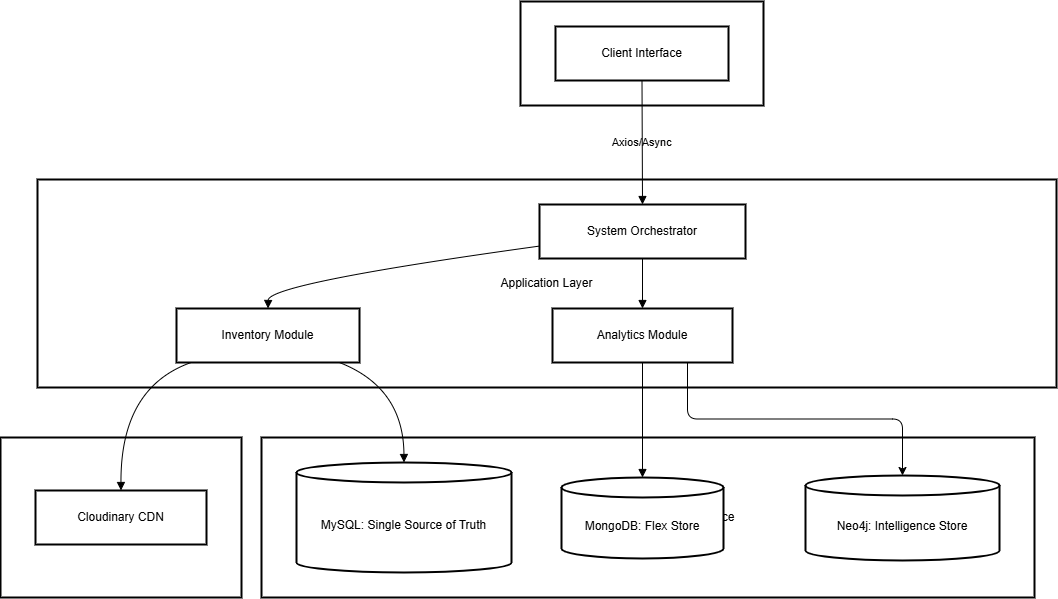
\includegraphics[width=1.0\textwidth]{screenshots/Architecture.drawio.png}
    \caption{System Design: High-Level Polyglot Architecture}
\end{figure}

\section{Polyglot Persistence Strategy}
The project rejects the "One Size Fits All" database approach:
\begin{table}[h!]
\centering
\begin{tabularx}{\textwidth}{p{0.18\textwidth} p{0.24\textwidth} X}
\toprule
\textbf{Database} & \textbf{Primary Role} & \textbf{Application Benefit} \\
\midrule
MySQL & Master Transactional Store & Absolute safety for orders and payments. \\
MongoDB & Search Index & Instant discovery and AI content mirroring. \\
Neo4j & Intelligence Engine & Graph-based fraud detection and upsells. \\
Cloudinary & Media Store & Offloading high-res assets from the server. \\
\bottomrule
\end{tabularx}
\caption{Polyglot Persistence Strategy}
\end{table}

\chapter{Database Design and Data Management}
\section{MySQL: Relational Schema Design}
MySQL acts as the "Single Source of Truth." Entities are normalized to ensure zero data redundancy.

\begin{lstlisting}[language=SQL, caption=Core Relational Tables]
CREATE TABLE vehicles (
    vehicleid INT NOT NULL AUTO_INCREMENT,
    seller_userid INT,
    model VARCHAR(100),
    price DECIMAL(10,2),
    status VARCHAR(30) DEFAULT 'Available',
    -- ... other specs
    PRIMARY KEY (vehicleid)
);
\end{lstlisting}

\section{PL/pgSQL and MySQL Logic}
We move "Business Rules" into the database for performance and safety.

\subsection{Procedures: The 15-Year Rule}
The \texttt{find\_age} procedure ensures we do not pollute our marketplace with outdated vehicles.
\begin{lstlisting}[language=SQL]
CREATE PROCEDURE find_age(IN p_vehicleid INT)
BEGIN
    DECLARE v_age INT;
    SELECT TIMESTAMPDIFF(YEAR, dateofmanufacture, CURDATE()) INTO v_age FROM vehicles WHERE vehicleid = p_vehicleid;
    IF v_age > 15 THEN
        SIGNAL SQLSTATE '45000' SET MESSAGE_TEXT = 'Validation Error: Vehicle older than 15 years.';
    END IF;
END;
\end{lstlisting}

\subsection{Triggers: Atomic State Changes}
This trigger ensures a vehicle is marked as 'Sold' the moment an order is completed, preventing accidental double-buying.
\begin{lstlisting}[language=SQL]
CREATE TRIGGER after_order_status_change AFTER UPDATE ON orders
FOR EACH ROW
BEGIN
    IF NEW.status = 'Completed' THEN
        UPDATE vehicles SET status = 'Sold' WHERE vehicleid = NEW.vehicleid;
    END IF;
END;
\end{lstlisting}

\chapter{Graph and NoSQL Intelligence}
\section{Neo4j: Graph Intelligence}
Neo4j handles our most complex relationship problems.

\subsection{Fraud Detection Query}
This query identifies cases where a vehicle's mileage reading has been manipulated.
\begin{lstlisting}[language=SQL, caption=Odometer Anomaly Detection]
MATCH (v:Vehicle {id: $vId})-[:HAS_SERVICE]->(sr1:ServiceRecord),
      (v)-[:HAS_SERVICE]->(sr2:ServiceRecord)
WHERE sr1.date < sr2.date AND sr1.km > sr2.km
RETURN sr1, sr2;
\end{lstlisting}

\subsection{Recommendations Logic}
\begin{lstlisting}[language=SQL, caption=Frequently Bought Together]
MATCH (p1:Part {id: $pId})<-[:PURCHASED_PART]-(u:User)-[:PURCHASED_PART]->(p2:Part)
WHERE p1.id <> p2.id
RETURN p2.id, count(DISTINCT u) as strength ORDER BY strength DESC;
\end{lstlisting}

\section{MongoDB: Aggregation \& Filtering}
For the discovery UI, we use MongoDB aggregation pipelines to calculate real-time availability and ratings.

\begin{lstlisting}[language=Java, caption=Vehicle Discovery Pipeline]
db.collection('vehicles').aggregate([
    { $match: { price: { $gte: 10000, $lte: 50000 }, fueltype: 'Electric' } },
    { $sort: { price: 1 } },
    { $project: { model: 1, price: 1, age: { $subtract: [2024, "$year"] } } }
]);
\end{lstlisting}

\chapter{Application Experience}
The AutoTrade frontend is built with React and Vite to provide an ultra-responsive user interface across all three system roles. For a detailed visual walkthrough of the user interface, administrative panels, and service center tools, please refer to the comprehensive \textbf{Appendix A: Application Screenshots}.

\chapter{Conclusion}
The AutoTrade project demonstrates that the future of automotive commerce depends on the intelligent orchestration of multiple data models. By assigning mission-critical transactions to MySQL, discovery to MongoDB, and relationship intelligence to Neo4j, we have built a platform that is not only robust but also provides unparalleled trust and transparency to its users.

\appendix
\chapter{Application Screenshots}

\section{Administrative and Management Interfaces}
\begin{figure}[h!]
    \centering
    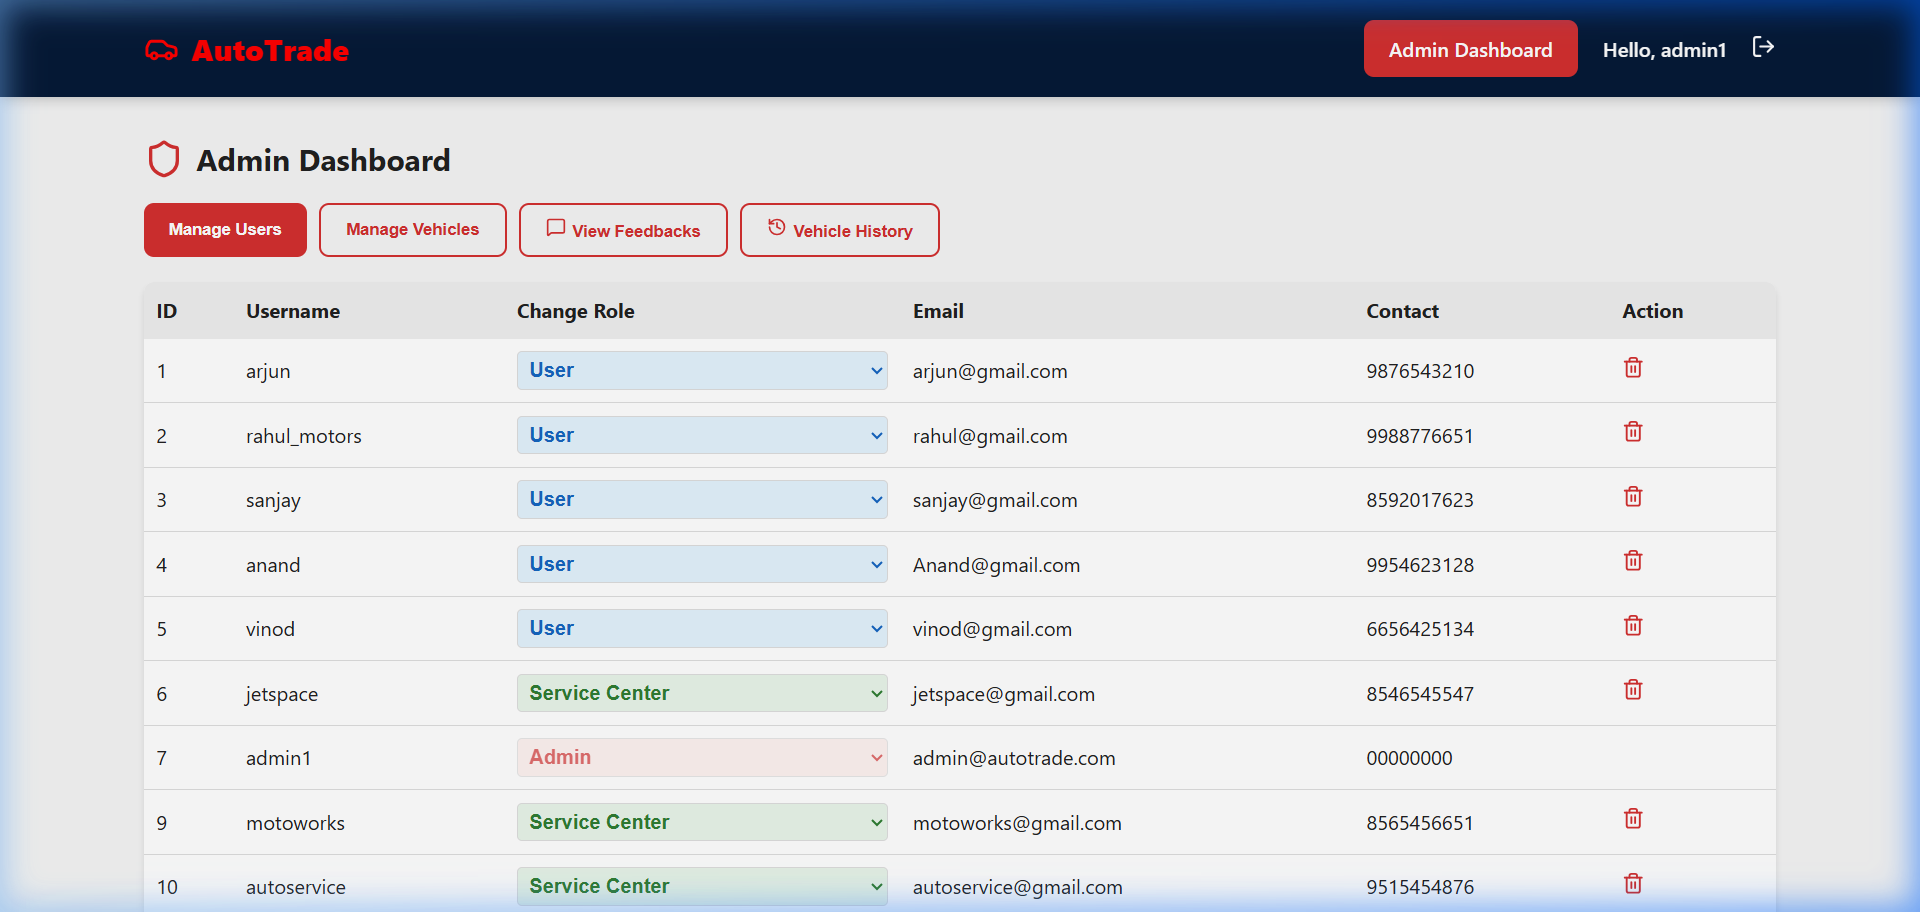
\includegraphics[width=0.8\textwidth]{screenshots/admin_dashboard.png}
    \caption{Admin Dashboard: Global Platform Oversight}
\end{figure}

\begin{figure}[h!]
    \centering
    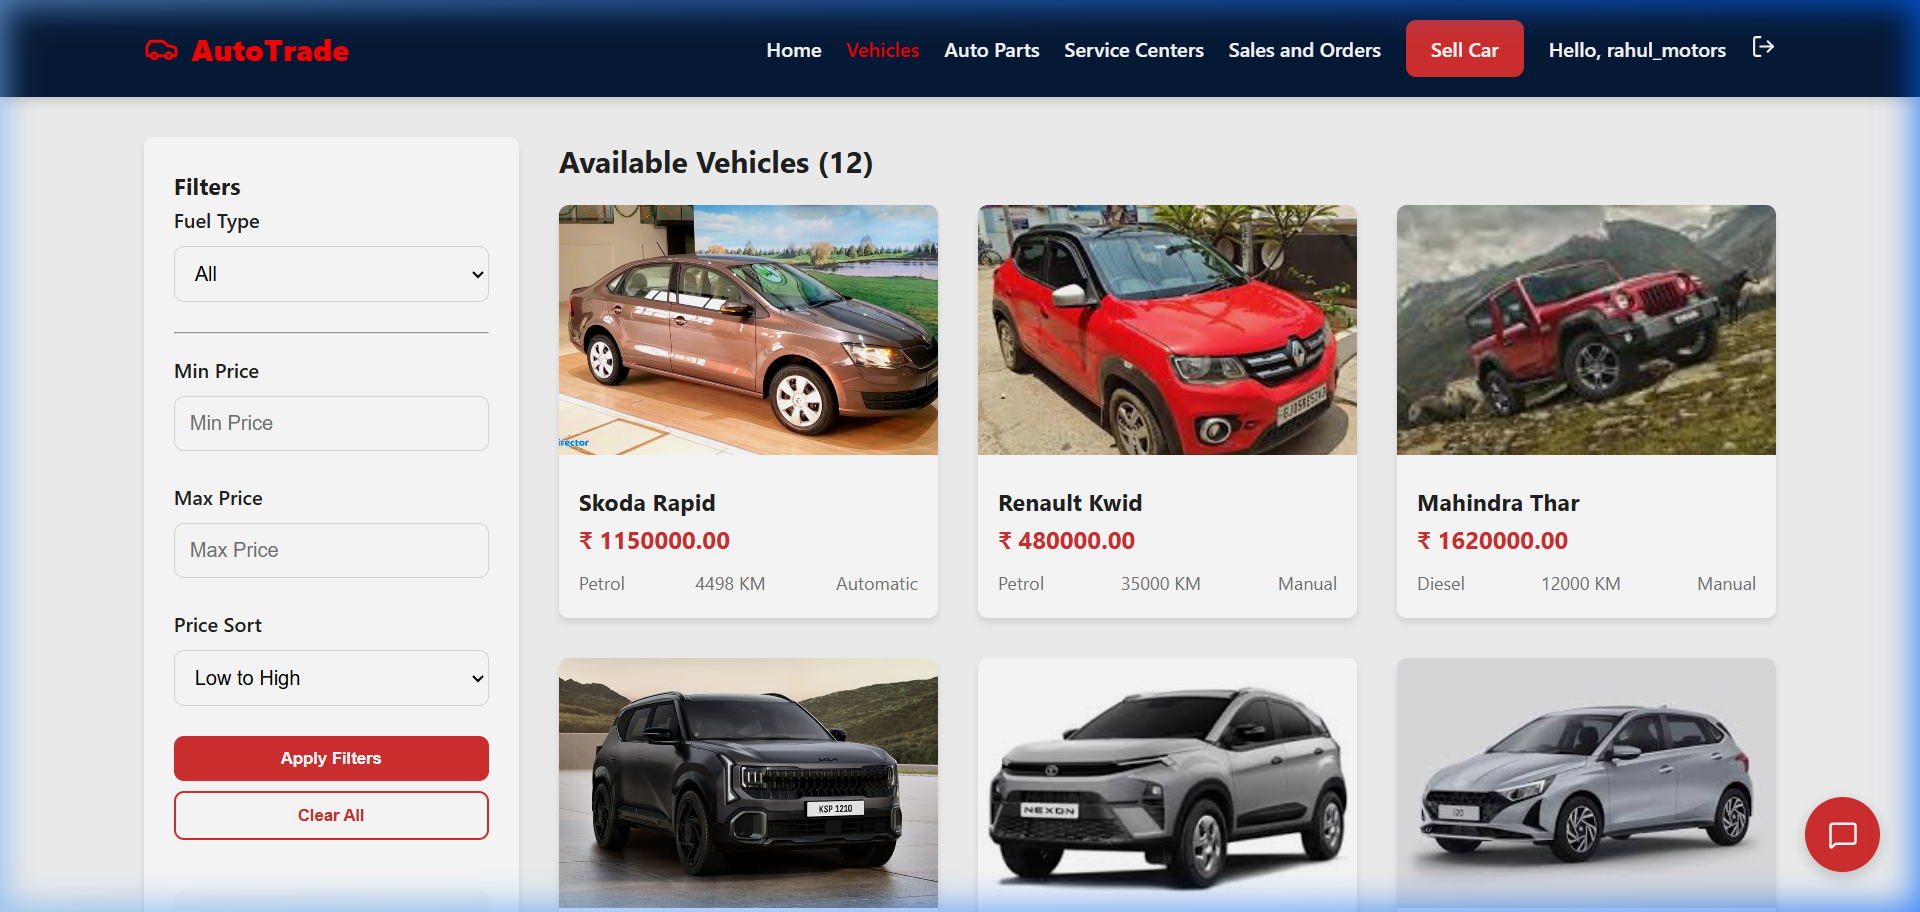
\includegraphics[width=0.8\textwidth]{screenshots/user_vehicles.png}
    \caption{Inventory Management: Seller View of Listings}
\end{figure}

\section{Consumer Marketplace Experience}
\begin{figure}[h!]
    \centering
    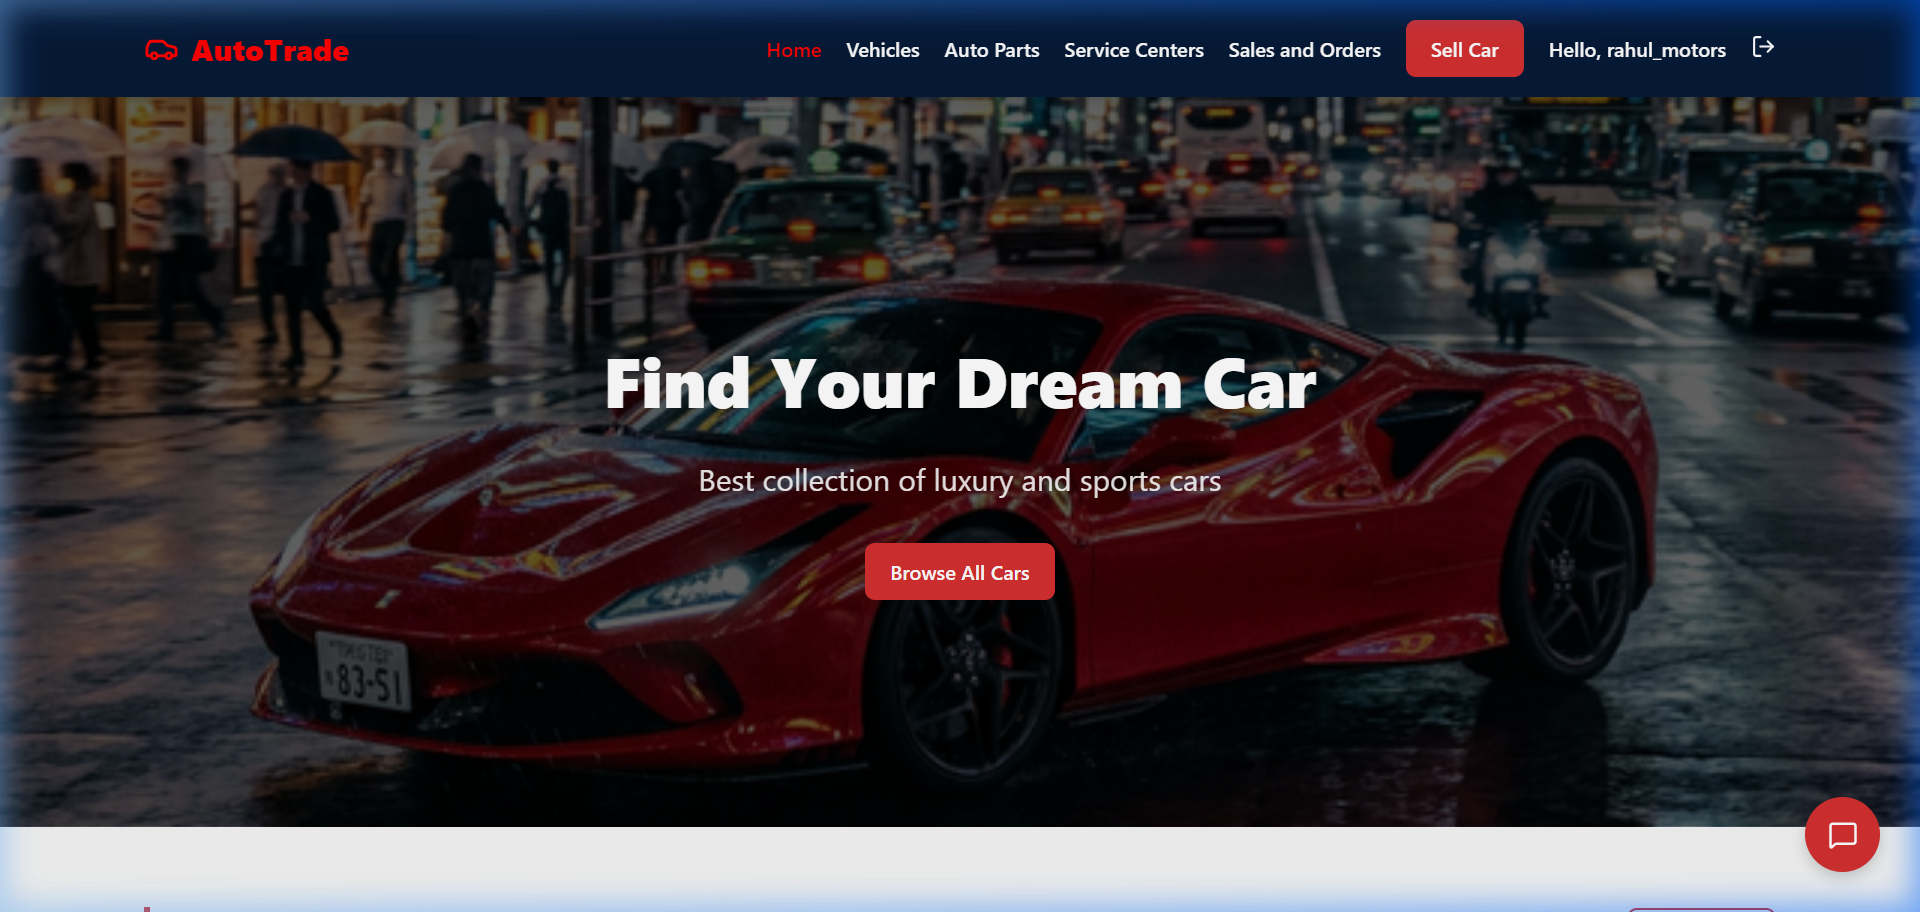
\includegraphics[width=0.45\textwidth]{screenshots/user_dashboard.png}
    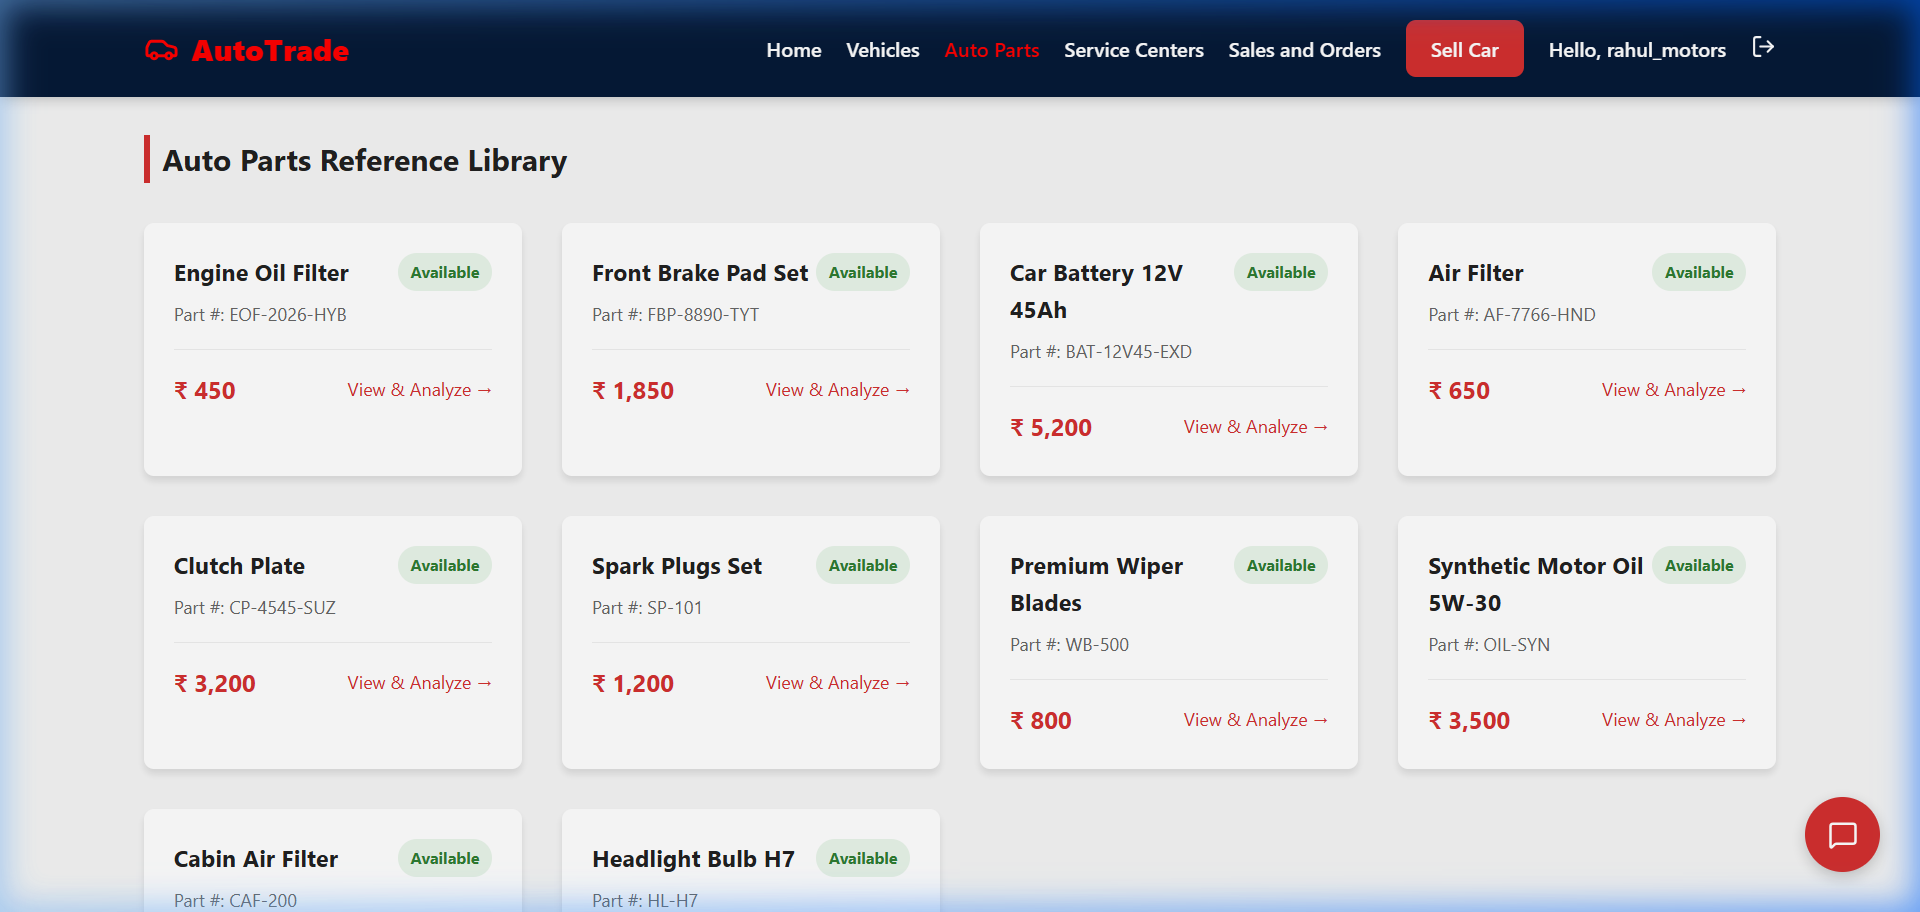
\includegraphics[width=0.45\textwidth]{screenshots/user_parts.png}
    \caption{User Dashboard and Multi-Media Storefront}
\end{figure}

\begin{figure}[h!]
    \centering
    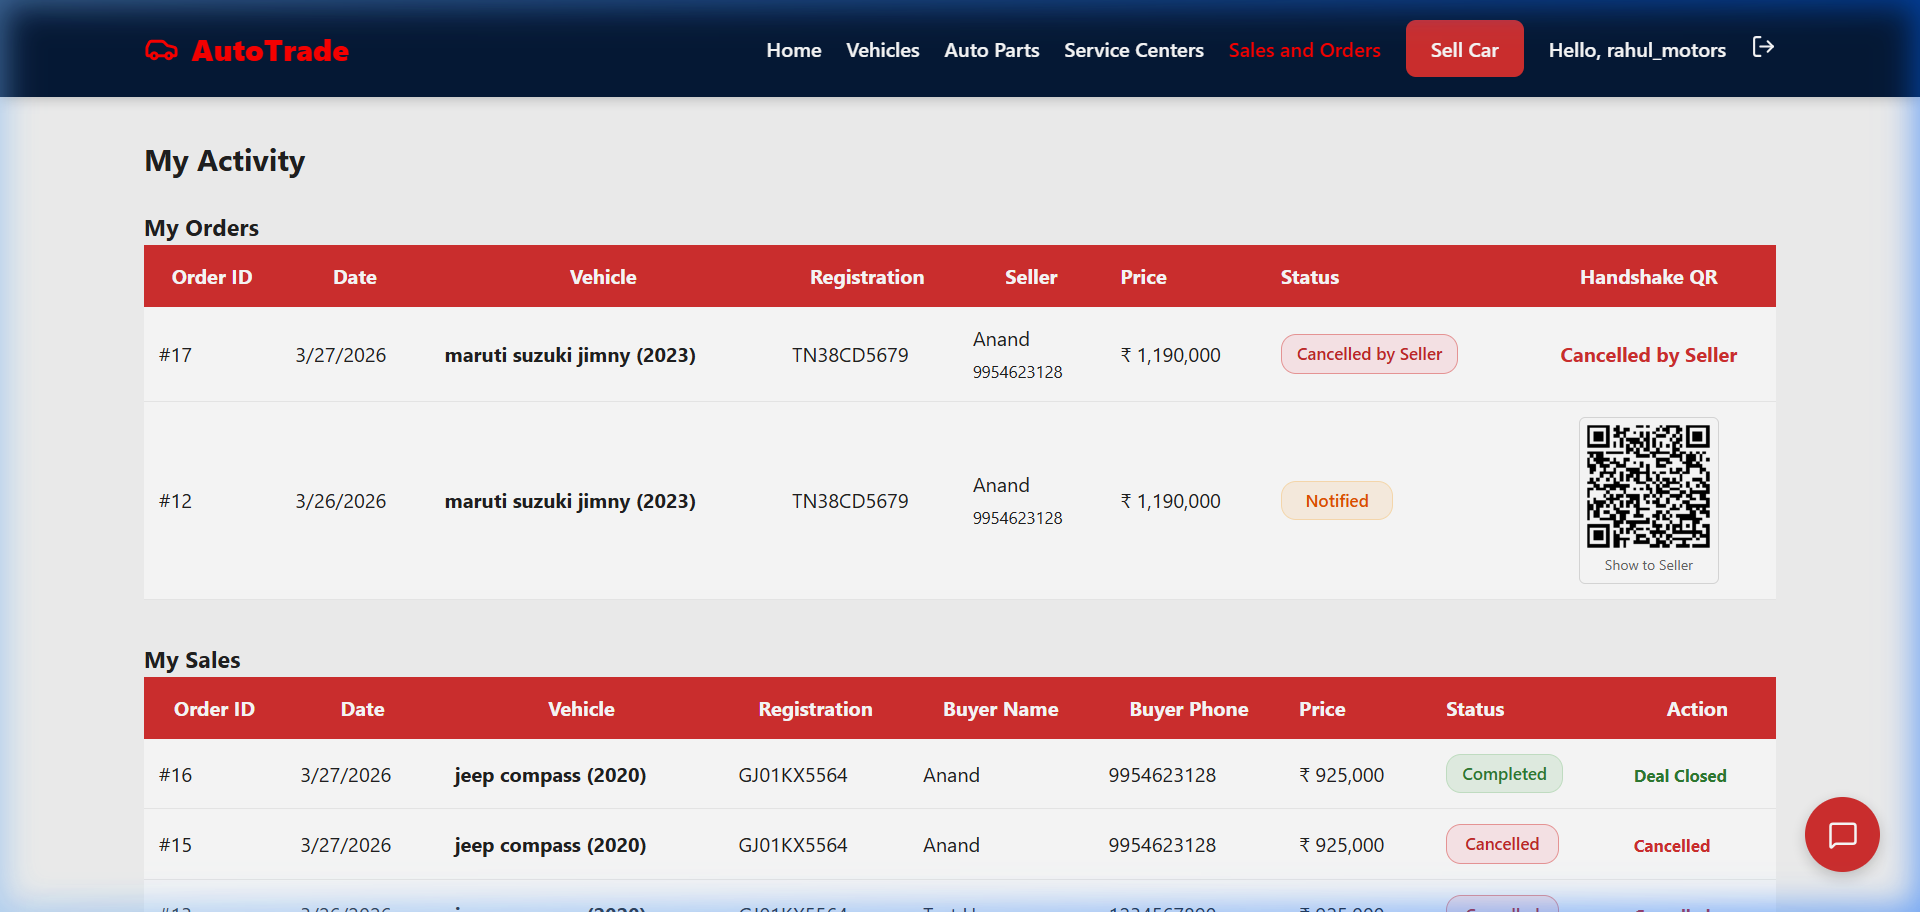
\includegraphics[width=0.8\textwidth]{screenshots/user_orders.png}
    \caption{Order History and Transactional Tracking}
\end{figure}

\section{Service Center Operations}
\begin{figure}[h!]
    \centering
    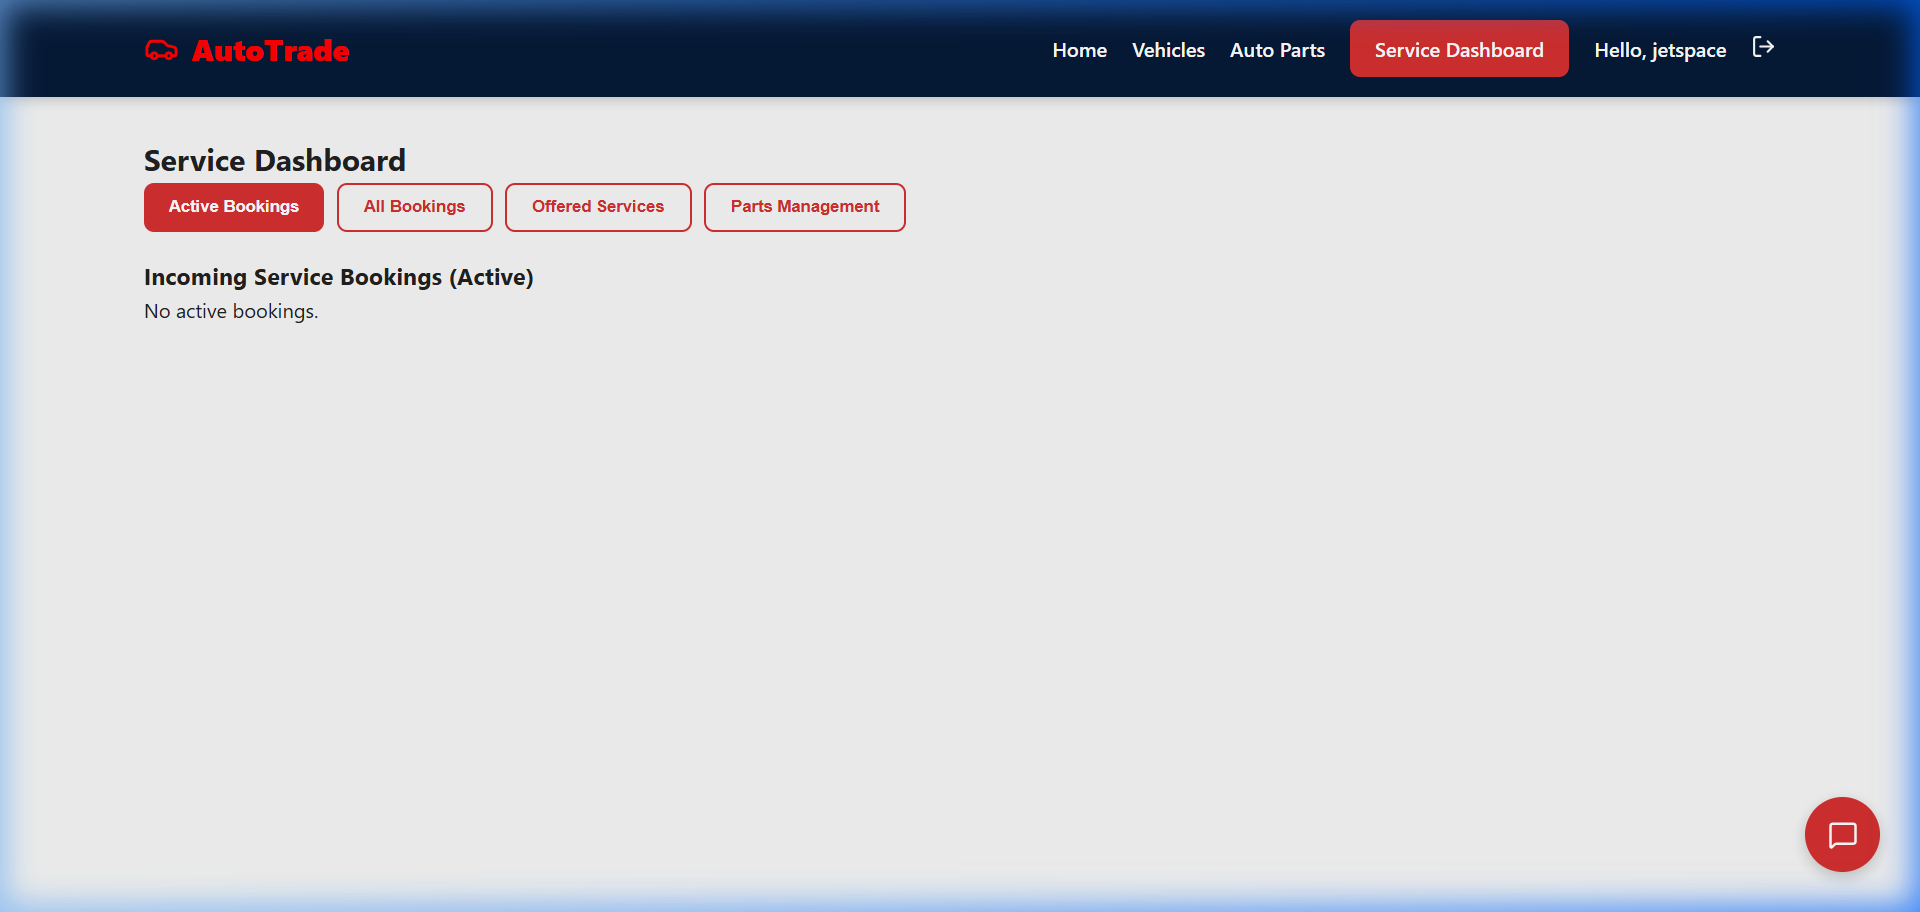
\includegraphics[width=0.45\textwidth]{screenshots/service_dashboard.png}
    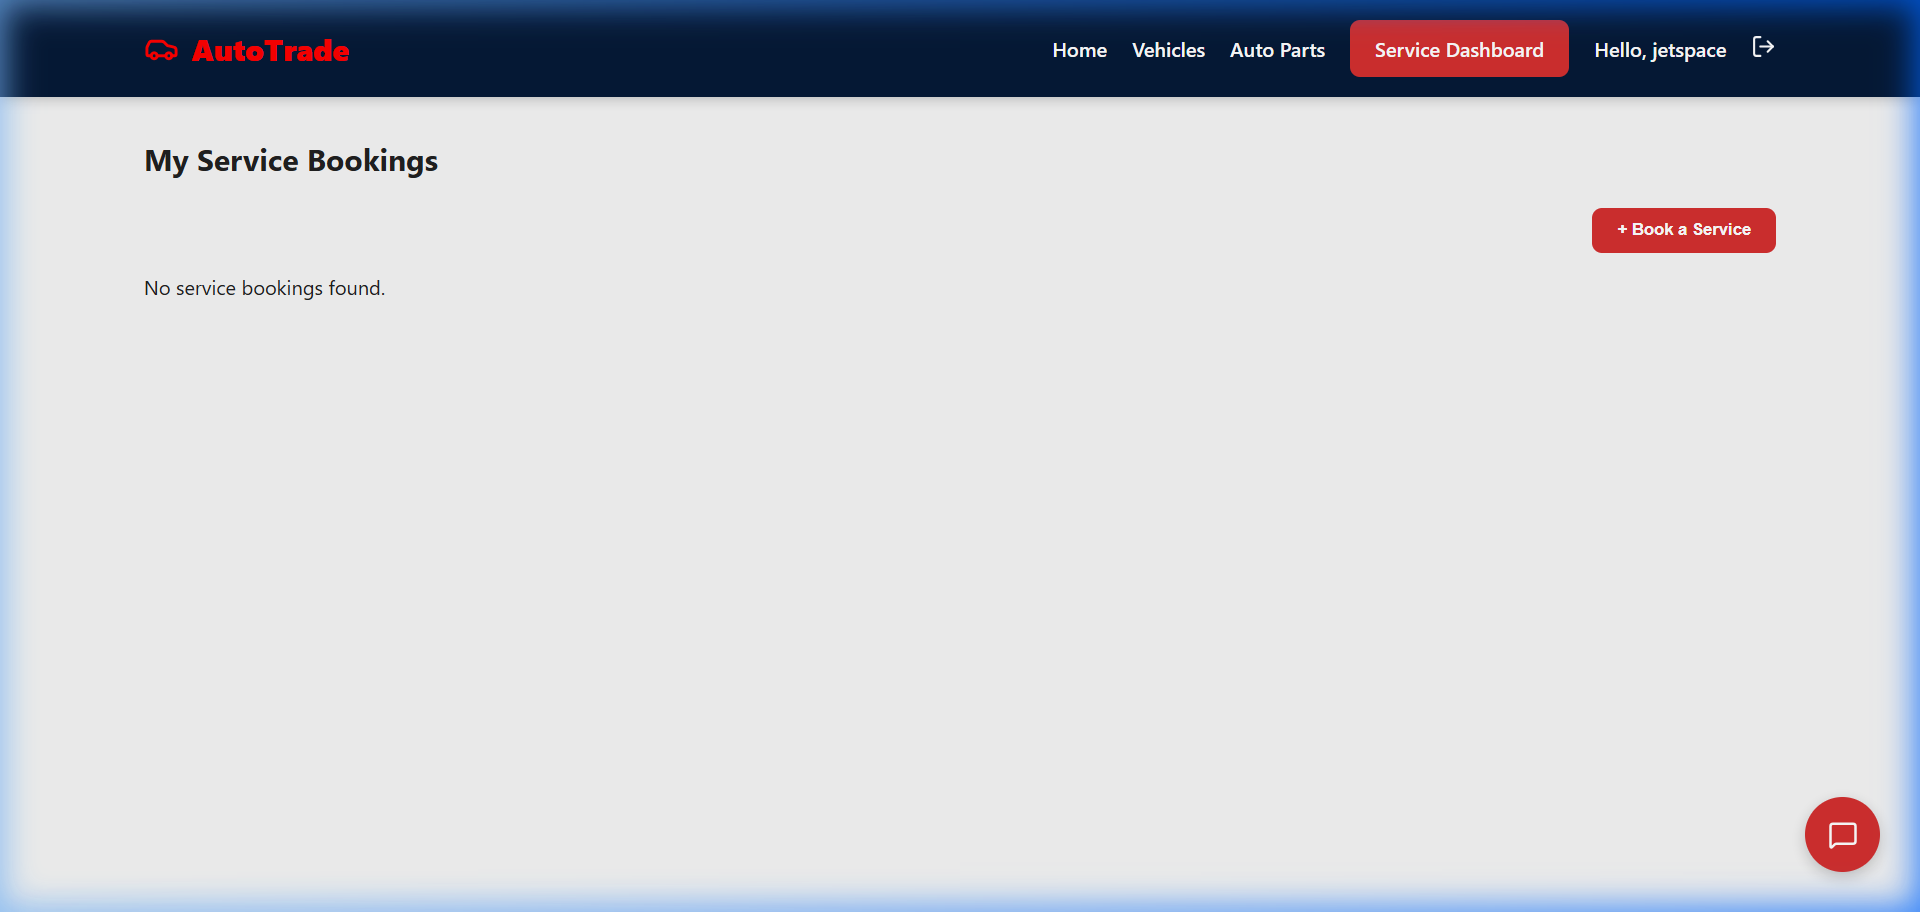
\includegraphics[width=0.45\textwidth]{screenshots/service_bookings.png}
    \caption{Service Provider Dashboard and Appointment Management}
\end{figure}

\end{document}
